\section{Dataset}\label{sec:dataset}

\begin{figure*}
	\centering
    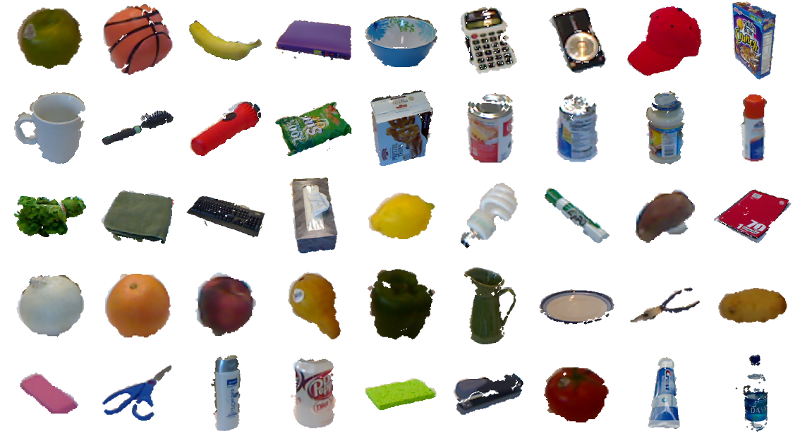
\includegraphics[width=0.8\textwidth]{images/rgbd_dataset}
    \caption{University of Washington's ``RGB-D object dataset''}
    \label{fig:rgb_dataset}
\end{figure*}

In this project, I use ``RGB-D object dataset'' from University of Washington \cite{Lai2011_rgbddata}. The dataset contains 200,000 samples (each is a collection of color and depth images, and a mask for background removal) of 300 household objects, divided into 51 categories (Figure \ref{fig:rgb_dataset}). Samples from the original dataset are recorded, synchronized, and aligned at the framerate of 30Hz and resolution of $640 \times 480$. However, I use a modified version of the dataset (also provided with the original one), where the objects are localized and cropped out. Each object is recorded on a turntable with three different camera viewpoints: low, middle, and high (Figure \ref{fig:apple_3_viewpoints}).

\begin{figure}
	\centering
	\begin{subfigure}[b]{0.3\linewidth}
	    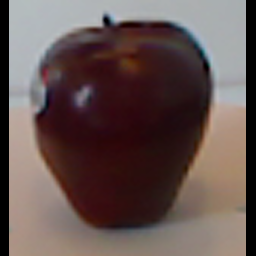
\includegraphics[width=\textwidth]{images/apple_1_1_1_crop.png}
    	\caption{}
	\end{subfigure}
    \begin{subfigure}[b]{0.3\linewidth}
	    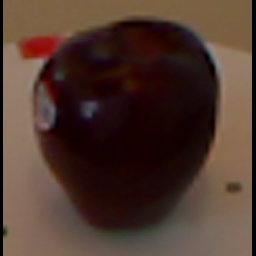
\includegraphics[width=\textwidth]{images/apple_1_2_1_crop.png}
    	\caption{}
	\end{subfigure}
    \begin{subfigure}[b]{0.3\linewidth}
	    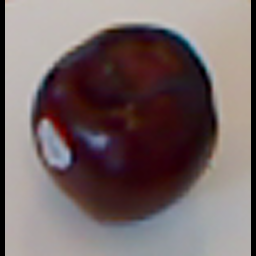
\includegraphics[width=\textwidth]{images/apple_1_4_1_crop.png}
    	\caption{}
	\end{subfigure}
    \\
    \begin{subfigure}[b]{0.3\linewidth}
	    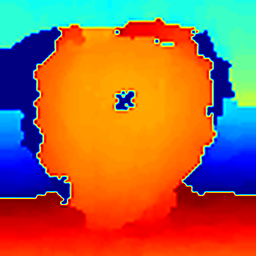
\includegraphics[width=\textwidth]{images/apple_1_1_1_depthcrop.png}
    	\caption{}
	\end{subfigure}
    \begin{subfigure}[b]{0.3\linewidth}
	    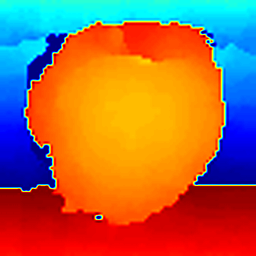
\includegraphics[width=\textwidth]{images/apple_1_2_1_depthcrop.png}
    	\caption{}
	\end{subfigure}
    \begin{subfigure}[b]{0.3\linewidth}
	    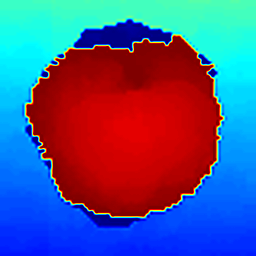
\includegraphics[width=\textwidth]{images/apple_1_4_1_depthcrop.png}
    	\caption{}
	\end{subfigure}
    \caption{Color and (visualized) depth images of an apple from 3 different camera viewpoints.}
    \label{fig:apple_3_viewpoints}
\end{figure}

University of Washington provides another dataset for evaluation. This dataset is constructed as the subset of the original one, keeping one sample out of every five. Samples in this set also have their backgrounds removed. The evaluation set comes with a list of 10 trial, each of which is a split of the dataset for evaluation. For each trial, one object per category is selected for validation, leaving the other objects of the same class for training. Since there are 300 objects and 51 categories, there are 51 objects for evaluation and 249 for training. For the sake of simplicity, I use only the first trial throughout this project's experiments.